\section{Ape 1}

\subsection{Vrai ou Faux}
Rappel : Un graphe simple est un graphe
\begin{itemize}
\item sans arêtes multiples
\item sans boucles
 \end{itemize}
\begin{enumerate}
	\item{L'élimination d'un sommet de degré maximum peut augmenter le degré moyen d'un graphe.}
	\item{Un graphe qui ne contient pas de triangle est biparti}
	\item{Deux graphes qui possèdent un même nombre de sommets et dont les listes de degrés sont identiques sont isomorphes. Même question, si, en plus, les graphes sont connexes.}
	\item{Un graphe simple de 2 sommets au moins possède toujours 2 sommets de degré identiques}
	\item{$\exists$ un graphe simple dont les degrés des sommets sont $\{1,2,2,3,3,4\}$}
	\item{$\exists$ un graphe simple dont les degrés des sommets sont $\{1,1,1,2,3,4,6\}$}	
\end{enumerate}

\begin{solution}
\begin{enumerate}
\item{
$d_{moyen} = \frac{\sum_{1}^{n} d_{i}}{n} \qquad d_{1} \leq d_{2} \leq ... \leq d_{n}$\\
Si on retire $d_{n}$ :
$d_{moyen} = \frac{1}{n-1}  (\sum_{1}^{n} d_{i} -2d_{n}) \qquad \stackrel{?}{>} \qquad \frac{\sum_{1}^{n}  d_{i}}{n}$\\
$\sum_{1}^{n} d_{i} - 2d_{n} \qquad > \qquad \frac{n-1}{n} \sum_{1}{n} d_{i}$\\
$\sum_{1}^{n} d_{i}(1- \frac{n-1}{n}) \qquad > \qquad 2d_{n}$\\
$\implies \qquad \sum_{1}^{n} d_{i} \qquad > \qquad 2n d_{max}$ Impossible !\\
Faux
}
\item{Faux, il peut avoir un cycle de longueur impair $\neq3$ (par exemple 5)}
\item{Faux :\\  
\includegraphics[scale=0.3]{graph_ape1_ex1_3_1}
$ \stackrel{Isomorphe}{\nRightarrow}$
\includegraphics[scale=0.3]{graph_ape1_ex1_3_2}
}
\item{Vrai}
\item{Faux - \textit{Théorème poignée de main} - La somme des degrés est impaire}
\item{Faux, le nœud de degré 6 est relié à tous les autres, donc le nœud de degré 4 et celui de degré 1 ne peuvent pas exister dans ce graphe.}
\end{enumerate}
\end{solution}

\subsection{Démontrez}
\begin{enumerate}
\item{D'un sommet de degré impair, $\exists$ toujours un chemin jusqu'à un autre sommet de degré impair.}
\item{Pour un graph simple et connexe de n sommets, on a $(n-1) \leq |E| \leq \frac{n \times (n-1)}{2}$}
\item{Un graphe simple qui possède plus de $\frac{(n-1) \times (n-2)}{2}$ arêtes est connexe.}
\item{Tout graphe qui possède n sommets et k arêtes possède au moins $n-k$ composantes connexes}
\end{enumerate}

\begin{solution}
\begin{enumerate}
\item{Soit un graphe connexe (pour un graphe non-connexe il suffit de considérer ses composantes connexe). Par le théorème des poignées de mains, $\sum deg(u_i) = 2 |E|$. Dés lors si le graphe possède un sommet de degré impair, il en possède forcément un autre. Et comme le graphe est connexe, toute paire de nœuds peuvent être reliés par un chemin, en particulier nos deux nœuds de degré impaire peuvent être reliés par un chemin.}
\item{
	\begin{itemize}
	\item Le graph étant connexe, il y a au minimum $n-1$ arrêtes.
	\item Le graph (connexe) étant complet, il y a maximum $\frac{n (n-1)}{2}$ arrêtes car on a:
		\begin{itemize}
		\item $n$ nœuds
		\item $n-1$ arrêtes par nœuds
		\item et donc $n (n-1)$ arrêtes $\times \frac{1}{2}$ car on les comptes deux fois!
		\end{itemize}
	\end{itemize}	
}
\item{ Essayons de construire le graphe non-connexe avec le plus d'arrêtes possibles. Ce faisant on construit le graphe composé de $K_{n-1}$ et d'un nœud isolé $u$. On a bien $\frac{(n-1)(n-2)}{2}$ arrêtes. Si on ajoute une arrête de plus, c'est forcément entre $u$ et $K_{n-1}$.	
	}
\item{Pour construire le graphe avec le moins de composantes connexes possible, il faut construire un arbre : on contruit une chaîne de noeuds. Avec $k$ arrêtes on peut relier $k+1$ noeuds. Cela nous donne $(n-k-1)+1=n-k$ composantes connexes.}
\end{enumerate}
\end{solution}

\subsection{Graphe de l'hypercube}
Soit $G_{i}$ le graphe dont les sommets sont des k-tuples de 0 et 1. Deux sommets de G sont adjacents si leurs k-tuples ne diffèrent qu'en une seule position. Montrez que le graphe est biparti, k-régulier et donnez son nombre arrêtes.\\

\begin{solution}
\begin{minipage}{0.35\textwidth}
\begin{flushleft}
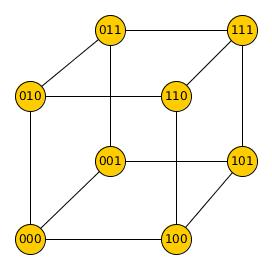
\includegraphics[scale=0.4]{graph_ape1_ex3}
\end{flushleft}
\end{minipage}
\begin{minipage}{0.65\textwidth}
\begin{flushright}
\begin{itemize}
\item Le graph est $k-régulier$ car tout les nœuds sont de degré k.
\item Le graph est biparti car $|E| = \frac{2^{k} k}{2} = 12$
\end{itemize}
\end{flushright}
\end{minipage}
\end{solution}

\subsection{Parcours fermés}
Formule : $(n-1)^{k} + (n-1)(-1)^{k}$
\begin{enumerate}
\item{Comptez le nombre de parcours fermés de longueur k dans $K_{n}$ (L'ensemble des graphes complets avec n nœuds)}
\item{Comptez le nombre de parcours fermés de longueur k dans $K_{k,n}$ (L'ensemble des graphes bipartis avec n nœuds dans chacune des partitions)}
\end{enumerate}

\begin{solution}
\begin{enumerate}
\item
\item
	\begin{itemize}
	\item Exemple avec $n=3$ :\\
	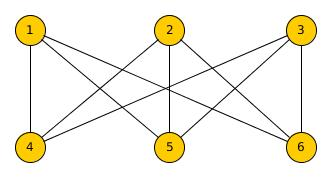
\includegraphics[width=0.4\textwidth]{graph_ape1_ex4}
	\item 
	 $A = \begin{pmatrix}
	 0&0&0&1&1&1\\
	 0&0&0&1&1&1\\
	 0&0&0&1&1&1\\
	 1&1&1&0&0&0\\
	 1&1&1&0&0&0\\
	 1&1&1&0&0&0\\
	 \end{pmatrix}$

	\item $|E| = \frac{n^{2}}{2}$
		
	\item $A^{k} $ donne le nombre de parcours.
	\item Si k est pair :
	 $A^{k} =  \left(
	 \begin{array}{c|c}
	 n^{k-1} & 0\\
	 \hline
	 0 & n^{k-1}\\
	 \end{array}
	 \right)
	 $
	\item Si k est impair :
	 $A^{k} =  \left(
	 \begin{array}{c|c}
	 0 & n^{k-1}\\
	 \hline
	 n^{k-1}&0\\
	 \end{array}
	 \right)
	 $
	\item $A_{i,j}$ Le nombre de parcours de $i \rightarrow j$. Il faut prendre les valeurs où $i = j$ pour obtenir le nombre de parcours fermés
\end{itemize}
\end{enumerate}
\end{solution}

\subsection{Trouvez le nombre de parcours de longueur k du sommet A à lui-même.}
\includegraphics[scale=0.5]{graph_ape1_ex5}


\subsection{Démonstration - Les rois du graphe}
Un tournoi de n joueurs est un graphe complet $K_{n}$ dans lequel on a choisi une direction pour chaque arête. $\exists$ une arête $(u,v)$ lorsque u a remporté sa partie contre v. Un sommet u d'un tournoi est un roi si quel que soit le sommet v du graphe, il y a une arête $(u,v)$ où il a une arête intermédiaire w et des arêtes $(u,w)$ et $(w,v)$.

Prouvez qu'il existe toujours au moins un roi.
Utiliser ce résultat pour montrer que dans le cas où aucun sommet n'a un degré entrant nul, il y a toujours au moins 2 rois.
\begin{solution}
\begin{itemize}
\item S'il n'y a pas de cycle, il suffit de remonter à l'origine pour trouver le roi.
\item S'il n'y a pas de cycle, il y a plusieurs rois. 
\end{itemize}

Dans la deuxième partie, on est dans le cas d'un cycle.\\Ce graph est un exemple o il y a 3 rois. \includegraphics[scale=0.5]{graph_ape1_ex6}\\

\end{solution}

